\documentclass[sigconf]{acmart}
\usepackage{pgfplots}
\pgfplotsset{compat=1.18}

\begin{document}

\title{725 Progress Report}
\author{Marie Mellor \and Clinten Hopkins \and Danny Gardner}

\maketitle


\section{Literature Report}
   % Kind of like the related works section of a paper
   We focused on the comparisons between Sinew and the modern database services MongoDB, and PostgreSQL JSON. Our goal in doing this is to see how Sinew compares to modern database systems in aspects such as batch loading, querying, updating and overall performance and scalability. This section will cover the primary works used in our evaluation.

   \subsection{Sinew}

   The main objective of Sinew \cite{Tahara_Diamond_Abadi_2014} is to enable developers to be able to represent data using self-describing formatting while still utilizing SQL and other traditional database systems. It was built to be a middle layer between multi-structured data and a relational database management structure (RDBMS). Sinew acts as an efficient tool able to convert semi-structured data into something stored and maintained in an RDBMS.

   The Sinew system architecture consists of two layers, the use layer and the storage layer. The storage layer allows Sinew to manage and query multi-structured data efficiently. Sinew's schema supports universal relations in which one document corresponds to one row. For every key, value pair from a document, the value will logically get stored in the row and column which corresponds to the document and key. A hybrid approach was used for mapping logical to physical schema to maintain performance benefits, space efficiency and single column serialization. The approach consisted of a combination of "all-physical-column" approach and "all-virtual-column" approach. Using this new hybrid approach, columns for some of the attributes get created while the rest are stored in a special serialized column called the column reservoir. This enables Sinew to maintain the benefits of using physical columns where they're needed while still keeping less frequently accessed keys stored virtually.

   Sinew documents the attribute names, types and storage methods to maintain a correct mapping between logical and physical and make system optimizations possible in a catalog. This catalog keeps track of which keys have been observed, the key type information which has been derived from the data, the number of occurrences of each key, if a column is virtual or physical and a 'dirty' flag. The catalog is split into two parts so Sinew can easily identify logical schema and physical schema.

   A scheme analyzer is also used to allow Sinew to adapt to evolving data models and query patterns. This schema analyzer evaluates the current storage schema in order to determine a distribution of physical and virtual columns. This was done to minimize the overall cost of materialization while still maximizing increasing performance rates.

   A column materializer was used to maintain dynamic physical schema by moving data between the column reservoir and physical columns. This materializer was created with the intent of it being a background process that would run only when there are resources available for it within the system. This is where the "dirty column" as previously mentioned comes into play. A dirty column is where some values for a key might exist in the reservoir while others exist in a corresponding physical column. These dirty columns make sure that dirty bits in a catalog are set for that specific column.

   Within the use layer, data is loaded in two steps: serialization and insertion. During the serialization step, the loader first parses each document, making sure that its syntax is valid. After the validation, the document is serialized into the proper format. During the serialization step, the loader also aggregates information about the keys within the dataset such as presence, type and sparsity. This information is then added to the catalog. During the insertion step, all the serialized data is placed into the column reservoir and the dirty flag is set to true in the respective columns. The column data is then moved to physical columns once the dirty bit is picked up which creates the newly loaded data. This was put in place so the system components would remain modular.

   Due to the nature of the hybrid storage, queries must match the physical schema; this is where a query rewriter comes into play. Here, queries are converted into an abstract syntax tree so that they can be validated and later sent to the storage layer to be executed. If any of the column references cannot be validated, the physical column is rewritten.


   \subsection{MongoDB}
   The architecture of MongoDB consists of many features that enable a strong and flexible database. MongoDB is a non-relational document oriented database management system that utilizes a document structure to store its data~\cite{Geeks4geeksMongo}. Similar to RDBMS tables, MongoDB uses collections to hold data within the database, the collections are able to store documents which have different fields. Collections in MongoDB are what stores the data whereas documents represent a specific record within a collection. Unlike SQL databases like MySQL, a document with a field that might not exist in the database does not cause any errors~\cite{Mongo-Medium}.
  
   As of 2014, MongoDB's default storage engine became WildTiger~\cite{Mongo-Medium}. WildTiger enabled two concurrent writes to update different documents in the same collection without the need for serialization. This feature that was not possible with the original release of MongoDB. The Binary-JSON (BSON) objects in WildTiger are compressed and stored in a hidden index where BSON pairs stores any recordIDs. This increases the performance greatly by reducing the number of I/O transactions.


   The process by which MongoDB scales its data is necessary in order to meet any growing demands of an application or database. MongoDB supports two types of scaling: horizontal and vertical~\cite{Mongo-scalability}. Horizontal scaling, or scaling down, is done by distributing the data across multiple nodes where each node is responsible for storing portions of the data. This is achieved by sharding, a mechanism that involves partitioning a database into smaller parts called 'shards'. These shards are hosted on a separate server forming what is known as a shard cluster. Vertical scaling, or scaling up, is the act of increasing the capacity of a single server by adding CPU, RAM, or other storage resources. In terms of MongoDB, this would mean upgrading the hardware to something more powerful. This may prove to be effective overall but has its own limitations.
  

   \subsection{PostgreSQL JSON}
    PostgreSQL architecture \cite{PostgresMedium} is a combination of shared memory, background processes, and data files. The shared memory contains a shared buffer, and a WAL buffer. The shared buffer is responsible for minimizing disk input/output so long as it is able to minimize contention when accessed by multiple users. The shared buffer needs to be large enough so that it may be accessed quickly. The shared buffer should keep any frequently used blocks as long as possible. The WAL buffer is used to store changes in the database temporarily in a WAL file. The four main process types that Postgres hosts are: Postmaster, background, backend, and client. The Postmaster process creates the backend processes for the client connections and is the overall parent process for the rest of the processes. The background processes all serve different functions and play a major role in database management. The backend process executes queries before returning the results to the user. This task is reliant on local memory.

    In terms of scalability, Postgres scaling\cite{Postgres-scalable} requires the understanding and proper implementation of PostgreSQL horizontal scaling as well as vertical scaling. PostgreSQL is kept accessible by high availability (HA) regardless of hardware failures or software crashes. This type of HA implementation requires replication, failover, load balancing and continuous monitoring.


\section{Accomplishments so far}
    \subsection{Sinew Implementation}
    The main task of this problem is updating the Sinew code to be compatible with modern systems. In the original paper's implementation of Sinew they used Postgres as the underlying database \cite{Tahara_Diamond_Abadi_2014}. Since the publishing of the paper in 2014 Postgres has seen significant updates, so we need to update the version of Postgres and ensure that the system still works. For this phase, we aimed at simply getting the system to run with the version it was created with (9.3.0). The Sinew repository includes multiple bash and make files that perform the initial setup, install the database, and perform some basic tests.

    The main challenge with implementing Sinew is the lack of documentation in the repository. The initial README file provided no information on how to configure, initialize, or run the system. This left us with a daunting task of having to parse through each file in the repository to understand its function and how it impacted the overall system. In addition to no overarching documentation, the plentiful bash files in the repository are similarly left undocumented, which forced us to analyze each file to understand each one's intended purpose and the order in which to execute these. As we have analyzed the original source code we have tried to remedy this situation and have been creating our own documentation for the repository, which will allow future users to reproduce our implementation easily.

    We updated the initialization and startup files so that the project can be run on a WSL Ubuntu Linux instance. After the changes to these files the necessary software is able to be installed on the instance and can build a test database hosted on postgres. At this current point we are waiting to update the test bash files as we are working on acquiring the necessary data files to be able to insert and view documents; this will be covered in the next subsection. Once we have the data files we will verify that Sinew is able to load, store, and interact with semi-structured data. Following this, we will update the underlying Postgres version and perform any modifications to the repository that are needed to allow Sinew to be updated to current standards.

    \subsection{MongoDB Benchmark}
    In the original paper the authors compared the implementation of Sinew against MongoDB and Postgres JSON. During this phase we also started configuring the MongoDB benchmark system. During these experiments the database systems were evaluated on their performance of varying queries from the NoBench NoSQL benchmark suite \cite{NoSQLBench}. This suite has been continually updated since the original publishing and will provide a viable benchmark dataset. We are currently working on getting an implementation of this suite running which will provide the datasets necessary for evaluating our database frameworks. This involves configuring data generation for a MongoDB database, which we will then extract the outputted JSON documents to use for Sinew and Postgres JSON respectively.

    At this current stage we are configuring the necessary files for NoBench to generate the files. The benchmark does provide some documentation on how to configure the necessary YAML file to run the system, but it is limited at best. We have implemented some basic configurations that perform generation of simple data, along with performing reads and writes on a MongoDB database. We are currently configuring a YAML file that provides the data records that were used in the original paper, which involves implementing multiple binding functions from the NoBench suite. Once this is completed we will be able to use the generated data on all the benchmark database systems for the performance comparison.

\section{Results}

\begin{figure}[!h]
\centering
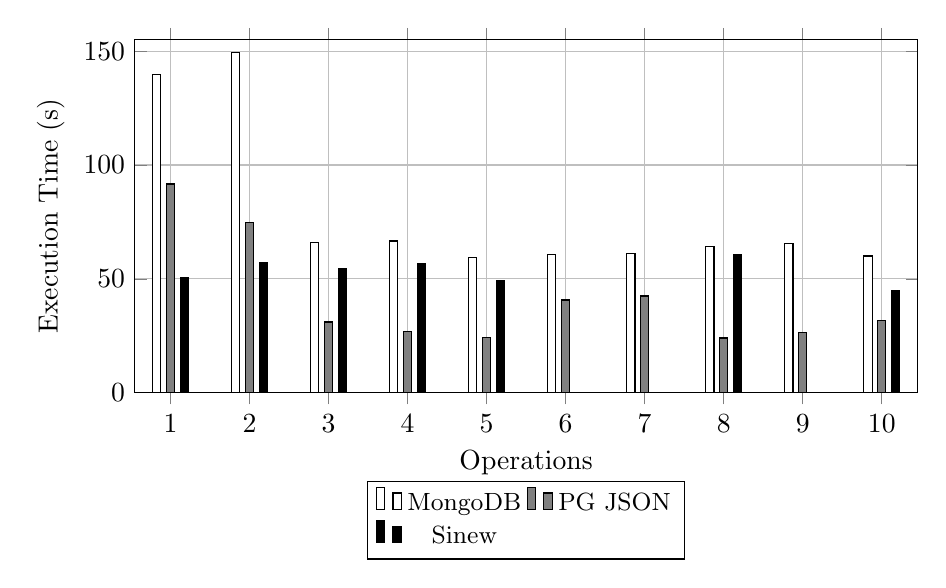
\begin{tikzpicture}
\begin{axis}[
    ybar,
    symbolic x coords={1, 2, 3, 4, 5, 6, 7, 8, 9, 10},
    xtick=data,
    xlabel={Operations},
    ylabel={Execution Time (s)},
    ymin=0,
    ymax=155,
    legend style={at={(0.5,-0.25)}, anchor=north, legend columns=2, font=\small},
    bar width=3pt,
    width=0.95\columnwidth,
    height=0.5\columnwidth,
    grid=major,
    enlarge x limits=0.05,
]

% Data for MongoDB
\addplot[fill=white] coordinates {(1, 139.8) (2, 149.4) (3, 66.0) (4, 66.6) (5, 59.4) (6, 60.6) (7, 61.2) (8, 64.2) (9, 65.4) (10, 60)};
\addlegendentry{MongoDB}

% Data for PG JSON
\addplot[fill=gray] coordinates {(1, 91.62) (2, 74.64) (3, 31.02) (4, 26.82) (5, 24.12) (6, 40.68) (7, 42.42) (8, 24.0) (9, 26.34) (10, 31.56)};
\addlegendentry{PG JSON}

% Data for Sinew
\addplot[fill=black] coordinates {(1, 50.52) (2, 56.94) (3, 54.6) (4, 56.58) (5, 49.14) (8, 60.84) (10, 44.94)};
\addlegendentry{Sinew}

\end{axis}
\end{tikzpicture}
\caption{NoBench Query Performance (Q1-Q10)}
\label{fig:results_chart}
\end{figure}

\begin{figure}[!h]
\centering
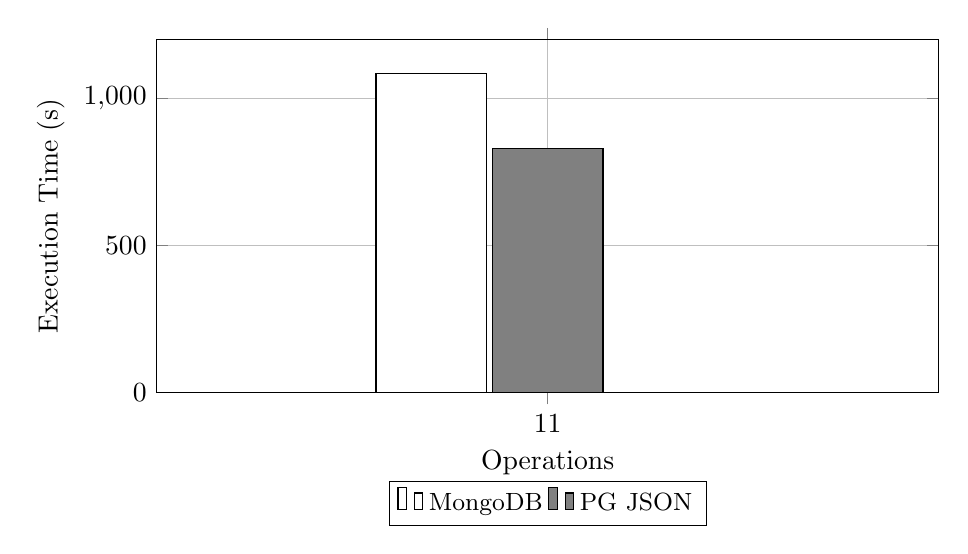
\begin{tikzpicture}
\begin{axis}[
    ybar,
    symbolic x coords={11},
    xtick=data,
    xlabel={Operations},
    ylabel={Execution Time (s)},
    ymin=0,
    ymax=1200,
    legend style={at={(0.5,-0.25)}, anchor=north, legend columns=2, font=\small},
    bar width=40pt,
    width=0.95\columnwidth,
    height=0.5\columnwidth,
    grid=major,
    enlarge x limits=0.05,
]

% Data for MongoDB
\addplot[fill=white, bar shift=-42pt] coordinates {(11, 1084.8)};
\addlegendentry{MongoDB}

% Data for PG JSON
\addplot[fill=gray, bar shift=+0pt] coordinates {(11, 829.8)};
\addlegendentry{PG JSON}

\end{axis}
\end{tikzpicture}
\caption{NoBench Query Performance (Q11)}
\label{fig:results_chart}
\end{figure}

\begin{figure}[!h]
\centering
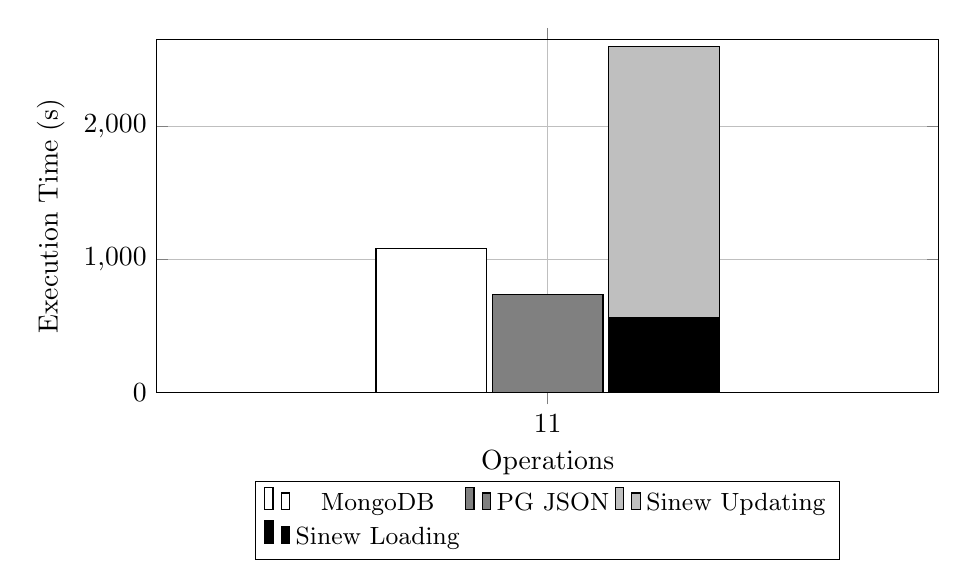
\begin{tikzpicture}
\begin{axis}[
    ybar, % Regular bar chart
    symbolic x coords={11},
    xtick=data,
    xlabel={Operations},
    ylabel={Execution Time (s)},
    ymin=0,
    ymax=2650,
    legend style={at={(0.5,-0.25)}, anchor=north, legend columns=3, font=\small},
    bar width=40pt,
    width=0.95\columnwidth,
    height=0.5\columnwidth,
    grid=major,
    enlarge x limits=0.4, % Adds space between grouped bars
]

% MongoDB Bar
\addplot[fill=white, bar shift=-42pt] coordinates {(11, 1084.8)};
\addlegendentry{MongoDB}

% PG JSON Base
\addplot[fill=gray, bar shift=+0pt] coordinates {(11, 734.35)};
\addlegendentry{PG JSON}

% PG JSON Base
\addplot[fill=lightgray, bar shift=+42pt] coordinates {(11, 2598.029413)};
\addlegendentry{Sinew Updating}

% PG JSON Additional (stacked on top of the gray bar)
\addplot[fill=black, bar shift=+42pt] coordinates {(11, 565.169413)};
\addlegendentry{Sinew Loading}

\end{axis}
\end{tikzpicture}
\caption{Load Time}
\label{fig:results_chart}
\end{figure}

\bibliographystyle{acm}
\bibliography{references}

\end{document}